\documentclass[a4paper,11pt]{kth-mag}
\usepackage[T1]{fontenc}
\usepackage{textcomp}
\usepackage{lmodern}
\usepackage[latin1]{inputenc}
\usepackage[swedish,english]{babel}
\usepackage{modifications}

\usepackage{csquotes}
\usepackage{graphicx}
\title{Machine Learning Applied to Playlist Generation}

\subtitle{Duis autem vel eum iruire dolor in hendrerit in
          vulputate velit esse molestie consequat, vel illum
          dolore eu feugiat null}
\foreigntitle{Lorem ipsum dolor sit amet, sed diam nonummy nibh eui
              mod tincidunt ut laoreet dol}
\author{Erik Aalto}
\date{Juni 2015}
\blurb{Master's Thesis at Spotify and CSC\\KTH Supervisor: Carl Henrik Ek\\Company Supervisor: Boxun Zhang\\KTH Examiner: Danica Kragic}
\trita{TRITA xxx yyyy-nn}
\begin{document}
\frontmatter
\pagestyle{empty}
\removepagenumbers
\maketitle
\selectlanguage{english}
\begin{abstract}
  This is a skeleton for KTH theses. More documentation
  regarding the KTH thesis class file can be found in
  the package documentation.


\end{abstract}
\clearpage
\begin{foreignabstract}{swedish}
  Denna fil ger ett avhandlingsskelett.
  Mer information om \LaTeX-mallen finns i
  dokumentationen till paketet.

\end{foreignabstract}
\begin{abstract}{Acknowledgements}
  I would like to thank ....surprise :)

\end{abstract}
\clearpage
\tableofcontents*
\mainmatter
\pagestyle{newchap}
\chapter{Introduction}

\section{Motivation}
Spotify today has more playlists than songs in their music library. Spotify also provides curated playlists as a form of music recommendation for their users. 

Given that a user has a preference for a specific playlist, an interesting feature would be to generate a playlist similar to the one a user has a preference for, but with different songs. This type of feature is interesting as it allows users to get music recommendations fitted to their needs. Such a feature could also give Spotify a competitive edge in the hardening competition for music streaming customers.

\section{What are Recommender Systems?}
Recommender systems provide an automated way to filter and rank information of interest for a certain user, possibly also taking time into account. A famous example of recommender systems is the product recommendation once initiated at Amazon, \textit{"Users who bought this product also bought"}. Another example of recommender systems are the movie recommendations provided by Netflix. Movie recommendations are interesting and non-trivial as a specific user at a certain time is likely to not be interested in the majority of movies provided by Netflix. The same thing applies to music, at any given moment a user is likely to not want to listen to the majority of songs in a music library . A last example of recommendation could be restaurant recommendation, where time and context are important factors. Recommending a simple hamburger restaurant is not likely to be of interest at date night, but it might be the perfect recommendation while driving the kids home after Saturday morning soccer game.

\section{What is Spotify?}
Spotify is a music streaming service which charges premium users a fee and presents free users with ads. Record companies are then paid according to the popularity of the tracks for which they hold digital rights. Spotify was launched in October 2008 and today has over 60 million active users, from which over 15 million are paying for the premium user service.

\section{Project Aim}
The aim of this thesis is to provide a scalable method for selecting candidate songs, in the context of playlist generation given a predefined playlist to mimic. This is an extension to the current field of music recommendation.  

\section{Limitations}
The work of this thesis is limited to finding candidate songs when generating playlists similar to Spotify \textit{Browse} playlists. The focus is on creating a scalable model of doing so. This means that any type of feature engineering is excluded from this thesis and the thesis is also limited from looking into the problem of ordering songs in playlist generation. 

\part{Theory}

\chapter{Computational Complexity}
Here goes an introduction to Big-O notation and why it is important in the context of recommendation.

\chapter{Basic Statistics}
Here goes arithmetic mean, geometric mean, variance, standard deviation, covariance, dot product

\chapter{Machine Learning}
Here goes cosine measure, PCA, LSH, subspace projections, clustering, generative vs discriminative models, curse of dimensionality, factor analysis, possibly some evaluation theory

\chapter{Background}

Previous work within the recommender system domain mainly focuses on two approaches. These are collaborative filtering and content based approaches. A hybrid of these two approaches can also be used. Both collaborative filtering and content based approaches typically try to infer a user ranking for a specific item\cite{melville2002content}. An item would in the context of music recommendation be a song, artist or album.

\section{Collaborative Filtering}
Collaborative filtering focuses on user's past behaviour. From this past behaviour of a specific user and past behaviour of similar users the ranking for the specific user for a certain item is inferred\cite{sarwar2001item}\cite{su2009survey}. In other words, a user gets recommendations of items that other users with similar taste like\cite{adomavicius2005toward}. Collaborative filtering suffers from something called the cold start problem, which occurs when the ranking for a specific item and user is inferred when there is no or little information of the current user behaviour\cite{herlocker2004evaluating}. Collaborative filtering has the advantage that it only relies on past user behaviour without the need of explicit user profiles. The fact that collaborative filtering only looks at user data means that it is domain free, i.e. the model is not dependent on whether users have rated books, movies, music or a combination thereof\cite{hu2008collaborative}.

Collaborative filtering can be used with explicit user feedback, such as the movie ratings used by Netflix, but it can also be used with implicit user feedback\cite{hu2008collaborative}. In the music context implicit feedback could be whether a song has been played or skipped.

An example of collaborative filtering applied to music recommendation is the recommender system used by last.fm. Collaborative filtering is also part of the music recommendation pipeline used in production at Spotify.

Collaborative filtering methods can be divided into two categories, memory-based and model-based. Memory-based collaborative filtering algorithms can be seen as user based while the model-based algorithms can be seen as item based\cite{sarwar2001item}.

Memory-based collaborative filtering algorithms operate on the entire user-item matrix where the full user history data set is used. The user-item matrix could for example consist of one user per row and one item per column. This data set is used to predict a preference for a previously unseen item for a specific user. To do this the rows most similar to the row corresponding to the specific user are found. The ratings of the users corresponding to these rows for the unseen item are then used to predict the rating for the specific user. As similar user's ratings are used to predict a specific user's rating memory-based models can also be thought of as neighbourhood models\cite{hu2008collaborative}. There are various ways implementing a memory-based model, but a naive way could be to find rows by using the cosine similarity and then simply averaging the rating of the top-n similar users for a specific item. This naive approach has a $O(MN^2)$ complexity where M is the number of users and N the number of items. One downside of this approach is that it does not scale very well when the user-item matrix is large. Another downside is that the user-item matrix is likely to be very sparse and using a nearest neighbour approach in this setting can lead to poor performance\cite{sarwar2001item}\cite{su2009survey}.

Model-based collaborative filtering means that the user history data is used to create a probabilistic model for ratings. At run time the model, rather than the entire user history data set, is used to make predictions of items for users. Model-based approaches are likely to scale better than memory-based ones\cite{sarwar2001item}. One approach to model-based collaborative filtering is to use latent factors. This means that each user would be associated with a user-factors vector $x_u \in R^f$ and each item with an item-factors vector $y_i \in R^f$. The predicted value of a user for an item would then be the inner product between the corresponding user and item vectors, i.e. $\hat{r}_{ui} = x_u^T y_i$. To avoid overfitting the model can be regularized, which means including a bias. A model as follows is then obtained: 
\begin{equation}
min_{x_*,y_*} \sum (r_{ui} - x_u^Ty_i)^2 +  \lambda(||x_u||^2 + ||y_i||^2)
\end{equation}

The problem with equation 5.1 is that it assumes knowledge of explicit feedback. In the context of music recommendation the case is rather that implicit feedback is available than explicit. What can be done in this case is to use binary labels expressing whether a user has preference for an item or not. Having preference for an item could mean that the user has streamed that song and not skipped it for example. Therefore the binary variable $p_{ui}$ is used to describe user preference.

There is however an uncertainty to the preference a user has. Has a user really preference for a song that come on Spotify Radio while the user was in another room? What can be done is to create confidence variables, that could depend on the number of times a song has been streamed. What can be done here is to use another variable \[ c_{ui} = 1 + \alpha r_{ui} \] where $r_{ui}$ is the number of times user \textit{u} has streamed item \textit{i}.

The resulting model then becomes:
\begin{equation}
min_{x_*,y_*} \sum c_{ui}(p_{ui} - x_u^Ty_i)^2 +  \lambda(||x_u||^2 + ||y_i||^2)
\end{equation}

Problems still remain as users and items can contain bias. The remedy is to enter bias terms, the resulting model is then:

\begin{equation}
min_{x_*,y_*} \sum c_{ui}(p_{ui} - x_u^Ty_i - b_u - b_i)^2 +  \lambda(||x_u||^2 + ||y_i||^2)
\end{equation}

Where $b_u$ is the user bias term and $b_i$ is the item bias term.

The resulting problem is a non-convex optimization problem, but by fixing either the user or item vectors the problem becomes convex and can be solved by the use of alternating least squares, where the cost function is guaranteed to get a lower value with each iteration\cite{hu2008collaborative}.

\section{Content Based Approaches}
Content based approaches for recommender systems recommend items that are similar to items  a user has had preference for in the past. This can be done by either comparing items to items or to create a user profile based on a users preferred items{adomavicius2005toward}. Content based approaches look at discrete features of items and tries to infer a similarity between two items given their similarity of features. A parallel can be drawn between content based recommendation and information retrieval.In the context of content based recommendation the cost function that is minimized is the distance between item.\cite{adomavicius2005toward}.

An example of a content based approach within music recommendation are the recommendations made by online radio station Pandora. 

Downsides with content based recommendation are that a user can never be recommended something that is not similar to what the user has expressed preferences before in the past. Further, content based recommendation is limited to the features of items. If the features used to describe items are poor a content based recommender system is likely to perform poorly. Lastly, content based recommenders do not take sequential information into account. Thus a well written news article is seen identical to the same article written backwards as they contain exactly the same words\cite{adomavicius2005toward}.

\section{Hybrid Systems}
OLOLOLOL

\chapter{Previous Work}
\section{Probabilistic Graphical Models for Playlist Generation}
Earlier attempts of playlist generation has been made by Microsoft Research. Ragno, Burges and Herley has made a model for playlist generation that can take any type of ordered playlist material, such as curated playlists or albums, as training data, and constructs an undirected graph between songs that are within the reach of a nth-order Markov model. In this graph nodes constitute songs and edges get their weights depending on how many times two songs fulfil the nth-order Markov property. Once this is done the undirected graph is converted into a directed graph where edges weight´s, the transition probabilities, are normalized by the sum of outgoing weights from each node. Once the undirected graph is made a playlist can be generated by selecting an initial seed song and simply performing a random walk in the graph. This model assumes that the connectivity between songs does not have to take order into account and that one can prevent playlist drifting by adding higher order Markov properties\cite{ragno2005inferring}. 

From a contextual playlist generation perspective a problem with the approach taken by Rango, Burges and Herley is that if you generate a playlist from a random walk you cannot chose the playlist context for the generated playlist on before hand. Another problem with the probabilistic graphical model approach to playlist generation is that the graph created during training phase only works for songs that are in the training data set. This model is not generalizable so you cannot get a similar playlist to a playlist you like, but with different songs.

\section{Gaussian Processes for Playlist Generation}
Another approach to playlist generation is to use gaussian processes, this approach has been taken by Platt et al, also at Microsoft Research. Here the authors try to learn a gaussian process prior from training data. This prior is then used together with a set of songs, for which a user has expressed preference, to generate a playlist given an initial seed song. In the training phase a blend of linear kernels is used to learn the relationship of meta data features among songs that come in sequence. The coefficients for each linear kernel is learnt by finding the coefficient that minimizes the difference between the empirical covariance between songs and the value given by the linear kernel. Empirical covariance is in this case as simple as whether the training data songs belong to the same album or not. Once the training phase is done the playlist generation phase consists of predicting the user preference for each song in a set of candidate songs, i.e. the f-star function in this case is the predicted user preference for a song. The f-star value is calculated by weighing the blend of linear kernels between a seed song and each candidate song with a factor. This factor is the sum of similarity between the initial seed song and each user preference song weighted by how central each user preference song is in the preference space. Playlist generation is then done by simply choosing the songs with highest f-star value\cite{platt2001learning}.

This model generalizes to new songs, but the user preference space is seen as one single space. This is a simplification of reality where a user preference space is probably divided into several categories, for example a workout preference space and a chill-out preference space, something the model provided does not take into account, which can be claimed as a weakness in terms of playlist context generation. Neither does the model take the ordering of songs into account.

\part{Method}

\chapter{Methodology}

\section{Problem Outline}
The problem this thesis is trying to solve is to select a number of songs given a predefined playlist so that the selected songs constitute a playlist similar to the predefined one. 

\section{Assumptions}
\begin{displayquote}
\textit{Without assumptions you cannot do machine learning} \\\\Ryan Adams
\end{displayquote}

The goal of the thesis is to generate playlists, similar to seed playlists choosen by the user. In order to do this there is a need for assumptions regarding playlists.

The first assumption for this thesis is that curated playlists, playlists made by professionals whose work is to create good playlists, suited for a specific context are suitable training data to create a model that generates playlists suited to the same playlist context.

The second assumption made is that features that belong to each track in a curated playlist contain enough information to create a representation of the context this curated playlist is made for.

The third assumption is that a playlist can be looked at as a good mixture of songs, i.e. there is an inherit variance in the playlist that defines it. This is a clear distinction from assuming that playlists only consist of songs similar to each other.


\section{Data}
From the Spotify hadoop cluster all available playlists where extracted and then filtered based upon whether they were created by Spotify playlist curators or not. Once playlists were filtered, feature data consisting of discrete values for genre, mood and tempo were added to each track within the selected subset of playlists.

\section{Pre-processing}
The selected data did contain track duplicates within playlists. These were removed as they would otherwise affect each playlist´s covariance of features.

\section{Exploratory Data Analysis}
To get an overview of whether features of tracks in a curated playlist relate to each other within the playlist correlation exploratory data analysis was made through plotting. More specifically correlation plots on a playlist level were made. The idea behind plotting correlations instead of covariances is that the magnitude of the correlation shows the strength of the linear relationship between features, while a covariance plot would be polluted should different features be on different ranges. By plotting correlations the problem of calculating correlations for features with zero variance, given a playlist context, emerged. Zero variance terms are a problem in the correlation setting as calculating the correlation for a zero variance term would imply dividing by zero, a mathematically undefined operation. This problem was solved by setting the correlation for feature relations with zero covariance to zero. It can be argued whether this is mathematically correct or not. But the approach can be motivated in this setting by the fact that plots are done to get an intuition of the data. A correlation of zero for features with zero covariance thus gives a better intuition of relationships in the data set compared to setting the correlation to one.

Performing plots of feature covariances of a playlist also shows whether there are linear realtionships among features in that playlist or not.

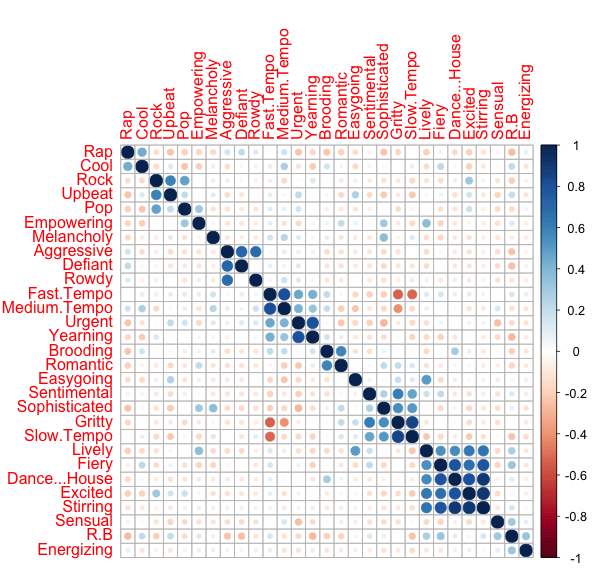
\includegraphics[scale=0.6]{images/0removedPlistFeaturePlot.png}

As we can see from the example plot above, there are clearly linear correlations among features for our example playlist.

\section{Learning Playlist Characteristics}
\begin{comment}
Motivate, why?
\end{comment}
Once that linear relationships have been spotted in the data the next step is to create a model that can learn the representation of a specific playlist. One simple approach to learning latent factors in data is principle components analysis, PCA.
Explaining the characteristics for a certain playlist context could be seen as equivalent of explaining the variance of features for tracks, given a curated playlist suited to the specific playlist context. Therefore extracting the main characteristics for a playlist context can be done by extracting the principal components, for the curated playlist representing that playlist context. It is reasonable to assume that the data that is modelled by PCA is not noise free, why PCA is performed up to a certain threshold for the variance explained and thus a dimensionality reduction is made. 
Using this approach extracting eigenvectors for the covariance matrix, rather than correlation matrix, is a motivated choice. The motivation behind this choice is that scaling the covariance matrix to a correlation matrix is a nonlinear transformation. If we want to use apply the principal components of a correlation matrix to the original data, then the original data need to undergo the same transform as transforming covariances to correlations. For a data set where each curated playlist makes up less than one percent of the total data it would be impractical to transform the original data over and over as we extract the principal components for each playlist context. Doing so would also not be feasible in terms of scalability. Using the covariance matrix for extraction of features is therefore motivated as the principal components of the covariance matrix can be directly related to the existing data.

\section{Handling zero variance terms}
Even though there are no zero variance terms in the whole data set, there are some terms that have zero variance within a certain curated playlists. These terms will not be handled by the principal components describing a playlist context, as principal components describe the variance of a playlist. Despite not being handled by the principal components zero variance terms might still have an important role in describing a playlist context. For example, if we have a curated jazz playlist then it is probably an important factor that all of the tracks in this playlist have a zero value for rap. The importance of this can be easily understood by imagining the opposite, what if those tracks would have a constant non-zero value for rap? Then a non-zero value for rap associated with jazz would be an important indicator for that playlist, why the absence must also be an important indicator.

\section{Selecting candidate songs for a playlist context}
The process of selecting candidate songs given a specific playlist context is an interesting and ambiguous problem without a given approach. Earlier work is focused mainly on item to item recommendation, i.e. recommending similar items of the same type given preferences for items of a certain times. But when it comes to selecting appropriate songs for a playlist context the items are of different kinds. The goal is to recommend songs, one type of item, given a playlist describing a playlist context, which is another type of item. 

One initial idea to select songs for a given playlist context could be that songs are either good candidates or not. This is a reasonable assumption, as for example for a rock classics playlist context then songs are either rock classics or not. Given that this is a binary classification problem, an efficient two class classifier might seem as a good idea at a glance. A support vector machine, SVM,  is an optimal two class classifier by definition, as a SVM maximizes the margin between classes\cite{cortes1995support}, and has the capability of multi class classification with for example the one versus all approach\cite{hsu2002comparison}. There is however one problem with support vector machines, or any classifier that requires training data within contextual playlist generation. The problem is that it is easy to define training data which labels a song as belonging or not belonging to a certain playlist. But it is hard to define what songs that belong to other playlists, than the one describing a specific playlist context, which are still relevant for that playlist context. For example a song belonging to a house Workout playlist may very well be a suitable candidate for a house party playlist. It is actually often the case that many songs belong to several playlists, describing different playlist contexts. Given this example a discriminative model turns out to be a bad fit for the problem this thesis is trying to solve. If a song belongs to a house party playlist then it is reasonable to assume that it would be outside the margin defining a house workout playlist if feeded to a SVM, even though this particular song might very well be a suitable match for the house workout playlist. This rules out the use of SVMs for the purpose of this thesis, as SVMs need to know the mapping between songs and playlist contexts to work. The same mapping that we are trying to find.

A second idea to selecting songs suitable for a specific playlist context would be to use centroid based clustering. The wikipedia definition of clustering is as follows: "clustering is the task of grouping a set of objects in such a way that objects in the same group (called a cluster) are more similar (in some sense or another) to each other than to those in other groups (clusters)". One could for example cluster all tracks in curated playlists and then simply assign each song that is not part of a curated playlist to the cluster providing the best fit for each track. But one problem is that there is not a one to one mapping between tracks and playlists, one playlist can contain many tracks and one track can belong to many playlists. This is different from clustering where each cluster consists of many points, but each point only belongs to one cluster, which yields centroid based clustering impropriate for the scope of this thesis. 

A third approach to finding candidate songs given a playlist context would be to tweak the normal usage of collaborative filtering. The common approach of collaborative filtering is to use a sparse matrix to infer the rating of items for one user given the ratings of similar users. What can be done instead is to use binary ratings and instead of inferring ratings for a user one could infer ratings for songs given a playlist. What this means is that playlists that contain the same songs as a playlist describing a playlist context one is interested in will be used to infer songs that are good matches for the specified playlist context. 

\subsection{Subspace method}
A last approach for track candidate selection would be to use the subspace method. Given that the principal components for a playlist, describing the variance of that playlist suited for a playlist context, are at hand, one can simply treat each track as a vector rather than a point. Each vector can then be projected into the principal component space for that playlist context. The underlying assumption is then that points that have a low relative change in magnitude under projection are well described by the characteristics defining the playlist context, and thus good candidates. Tracks that are not well described by the playlist context characteristics on the other hand, will change under projection and will therefore also have a high relative change in magnitude. There are however problems with this approach. Lets say that we have a playlist context that is defined by variance in the dimensions jazz, blues and rap and our vector space consists of the dimensions jazz, blues, rap and rock. If we then have a song that is characterized by jazz and blues only, then this song will go unchanged under projection. As the relative change in magnitude is none then this song will be suggested as a suitable candidate for the jazz, blues, rap playlist context. However a playlist context consisting of jazz, blues and rap is likely to be pretty peculiar and a song characterized by jazz and blues only is not likely to be a suitable match for such a playlist. Another problem would be songs that consists of zero values for all features, these songs would also go unchanged under any playlist context projection, but are not likely to be good candidates for all playlist contexts. Further, the subspace method is a linear transformation and it can be questioned if a linear transformation is powerful enough to describe the necessary mappings.

\section{First Track Manifold}
After studying linear relationships among features within playlists the study was extended to see if there were linear relationships among the ordering of songs as well. To do this the subspace method was used again. But instead of extracting the principal components for the variance of a playlist, the principal components describing the variance of all the start songs of all curated playlists were extracted. Once this was made a sample of songs from the curated playlist data set were projected into the first track manifold space created by the principal components of the first tracks. This was made to see if start tracks would have higher ranking, i.e. lower relative change in magnitude, than other tracks.

\section{Playlist Comparison}
As principal components were chosen to describe playlists, it is reasonable to assume that if principal components analysis works well for describing playlist characteristics, then the same approach should also work well for comparing playlists. Playlists were compared pairwise. To compare two playlists all eigenvectors from each playlist were multiplied by each other. By doing this the cosine measure of vector similarity for each pair of vectors was obtained. The problem with this approach is that it gives an unbalanced comparison. By simply looking at the similarity of eigenvectors implies that eigenvectors corresponding to low eigenvalues have the same importance as eigenvectors corresponding to high eigenvalues. For the reader uninitiated with eigenvalues this means that components explaining a high part of the characteristics of a playlist are regarded an equal importance as components explaining a low part of playlist characteristics. To remedy this problem the cosine score between eigenvectors from each playlist was scaled by the square root of the product of the corresponding eigenvalues. The result obtained from this multiplication was a matrix. To rank the similarity between these matrices some type of transformation from a matrix to a single value is needed. Several approaches were tested and are covered under the evaluation section.

\section{Approximate Nearest Neighbours}
OL

\part{Evaluation}

\chapter{Results}
OLOLOLOL

\chapter{Computational Complexity Analysis}
OLOLOLOL


\bibliography{refList}
\bibliographystyle{plain}

\appendix
\addappheadtotoc
\chapter{RDF}\label{appA}

\begin{figure}[ht]
\begin{center}
And here is a figure
\caption{\small{Several statements describing the same resource.}}\label{RDF_4}
\end{center}
\end{figure}

that we refer to here: \ref{RDF_4}
\end{document}
